\documentclass[10pt,twocolumn]{article}

\usepackage[letterpaper,margin=0.68in,columnsep=0.20in]{geometry}
\usepackage{amsmath,amssymb}
\usepackage{booktabs}
\usepackage{array}
\usepackage{enumitem}
\usepackage{graphicx}
\graphicspath{{figures/}{reports/figures/}}
\usepackage{xcolor}
\usepackage{hyperref}
\usepackage{url}
\usepackage{microtype}
\usepackage{float}
\setlength{\textfloatsep}{6pt plus 1pt minus 2pt}
\setlength{\floatsep}{6pt plus 1pt minus 2pt}
\setlength{\intextsep}{6pt plus 1pt minus 2pt}
\setlength{\abovecaptionskip}{3pt}
\setlength{\belowcaptionskip}{1pt}

\hypersetup{
  colorlinks=true,
  linkcolor=blue,
  citecolor=blue,
  urlcolor=blue
}
\setlength{\emergencystretch}{2em}
\setlist[itemize]{leftmargin=*,noitemsep,topsep=2pt}
\setlist[enumerate]{leftmargin=*,noitemsep,topsep=2pt}
\newcommand{\code}[1]{\texttt{#1}}
\urlstyle{tt}
\newcommand{\gcr}{GCR}
\newcommand{\kgtrie}{KG-Trie}
\newcommand{\dvi}{DVI}
\newcommand{\graphlite}{GraphLite}
\newcommand{\cwq}{CWQ}
\newcommand{\webqsp}{WebQSP}
\newcommand{\rogcwq}{RoG-CWQ}
\newcommand{\rogweb}{RoG-WebQSP}

\title{Constraint-Aware KG-Trie Reasoning for Knowledge-Grounded LLMs:\
DVI, GraphLite, and Embedding-Guided Path Selection}
\author{AIAA 4051 Final Research Project: Knowledge Grounded LLM Reasoner\\
Team Members: \emph{[fill in names]}\\
Project Manager: Jiujiu Chen}
\date{May 2026}

\begin{document}
\twocolumn[
\maketitle
\begin{abstract}
Large language models can answer complex questions, but their reasoning traces may contain unsupported facts. Graph-Constrained Reasoning (GCR) improves faithfulness by building a KG-Trie over knowledge-graph paths and constraining a KG-specialized LLM to generate only graph-valid reasoning paths. This project reproduces GCR, analyzes its failures, and implements three modifications to the graph-constrained reasoning pipeline: Decompose-Verify-Intersect (DVI), GraphLite, and embedding-guided KG-Trie construction. DVI adds a constraint-state controller: a general LLM decomposes a question into atomic constraints, a KG verifier collects per-constraint candidate sets, Python computes candidate intersections, and a confidence gate routes back to the GCR baseline when DVI evidence is unreliable. GraphLite replaces expensive KG-LLM verification with entity-level graph enumeration: relation selection, candidate-entity scoring, and selective two-hop expansion. Embedding-guided KG-Trie ranks candidate paths by question-path semantic similarity before trie construction and extends the path budget to preserve useful 3-hop evidence. On full RoG-CWQ, reproduced GCR reaches 54.55 F1 with Llama-3.1-8B, 54.50 F1 with Llama-2-7B, and 42.31 F1 with Qwen2-0.5B. Raw DVI alone underperforms the strongest baselines, but exact-size routed DVI improves Llama-3.1 from 54.55 to 54.63 F1 and Llama-2 from 54.50 to 54.51 F1, with oracle routing showing much larger headroom of 61.51 F1. GraphLite is substantially faster than KG-LLM DVI (3.09s vs. 12.72s per example) but lower quality (42.14 F1). Embedding-guided KG-Trie is close to Qwen GCR on full 2-hop evaluation and improves controlled 3-hop probes when paired with candidate reranking. The central conclusion is that KG path validity is necessary but not sufficient: complex KGQA needs explicit state for constraint satisfaction, answer typing, intersection, and temporal or numeric operators.
\end{abstract}
\vspace{0.6em}
]

\section{Introduction}
Knowledge graphs (KGs) store factual information as triples $(h,r,t)$ between entities and relation types. They are therefore a natural grounding source for knowledge-intensive question answering. A free-form LLM can generate plausible but false reasoning chains, while a KG-grounded system can restrict the model to evidence that exists in the graph.

The baseline for this project is Graph-Constrained Reasoning (GCR)~\cite{luo2025gcr}. GCR retrieves KG paths around question topic entities, serializes them into a prefix trie, and constrains a KG-specialized LLM so that generated reasoning paths follow graph-valid continuations. A final general LLM then reads those paths and produces answers. This design is strong because it attacks path hallucination directly.

The weakness is that a prefix trie represents linear path validity, not full constraint satisfaction. ComplexWebQuestions (CWQ) contains composition, conjunction, comparative, and superlative questions. Many examples require intersecting evidence from multiple entities, checking an answer type, applying a date or numeric filter, or choosing an argmax/argmin. A path can be perfectly KG-valid while still ending at a mediator node, ignoring a temporal predicate, or satisfying only one branch of a conjunction.

We study the following question: can KG-Trie reasoning be extended from local path validity to explicit multi-constraint answer satisfaction? We answer this through three implemented modifications:
\begin{itemize}
  \item \textbf{DVI}: decompose the question into atomic constraints, verify each constraint against the KG, intersect candidate sets programmatically, and route selectively between DVI and the original GCR output.
  \item \textbf{GraphLite}: replace token-level KG-LLM verification with explicit relation/entity enumeration, DeBERTa cross-encoder scoring, and selective two-hop candidate expansion, giving an efficiency-oriented verifier for DVI.
  \item \textbf{Embedding-guided KG-Trie}: rank paths by question-path semantic similarity before trie construction, allowing 3-hop evidence to be added without fully exposing the model to path explosion.
\end{itemize}

The project requirements ask us to reproduce the baseline, explore more than two KG-specialized LLMs, analyze failures by query type, and modify the graph-constrained decoding module for complex reasoning constraints. The report is organized around those requirements: baseline reproduction, failure diagnosis, three implemented reasoning modifications, experiments, and conclusions. Extra implementation paths and secondary tables are placed in the appendix so the main body stays near ten pages.

\paragraph{What changed relative to the baseline.}
The original GCR pipeline has two stages: a KG-specialized LLM generates constrained paths, and a general LLM turns those paths into answers. Our changes keep this overall interface but modify the evidence construction and verification layer. DVI inserts a controller around GCR and makes candidate-set intersection explicit. GraphLite keeps the DVI controller but swaps the verifier for explicit relation/entity enumeration and neural scoring. Embedding-guided KG-Trie keeps the baseline decoder but changes which paths enter the trie. These are deliberately complementary: one changes aggregation, one changes verification cost, and one changes retrieval coverage.

\paragraph{Why three methods are useful.}
The archive shows that no single modification dominates. DVI is closest to a reasoning-schema change and provides the best evidence for constraint-aware reasoning, but it needs a reliable router. GraphLite is faster and more inspectable, but weaker as a final QA system. Embedding-guided KG-Trie improves small 3-hop probes but not the full 2-hop Qwen baseline by itself. Reporting all three methods is therefore more honest than presenting one cherry-picked result: together they identify where the baseline fails and which parts of the solution are already working.

\begin{figure*}[t]
\centering
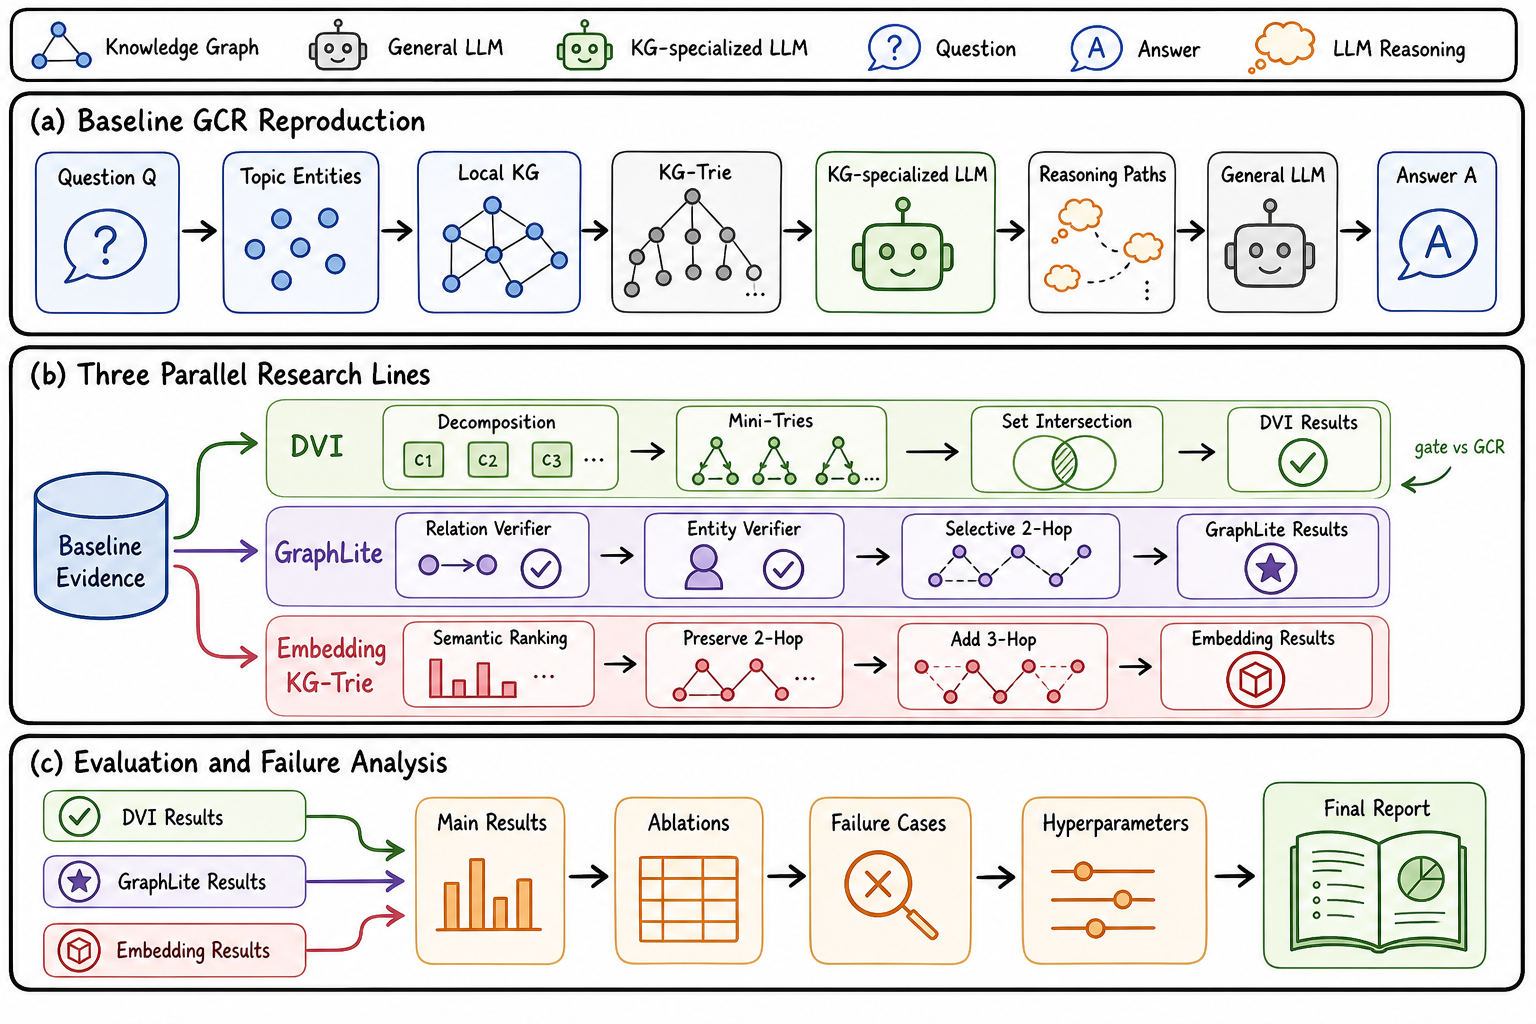
\includegraphics[width=\textwidth]{project_overview_handdrawn_gpt-image-2-v4.png}
\caption{Project overview in a hand-drawn research-figure style. The three modification lines, DVI, GraphLite, and embedding-guided KG-Trie, are parallel research directions evaluated against the reproduced GCR baseline; only DVI includes an internal gate against GCR.}
\label{fig:overview-architecture}
\end{figure*}

\section{Related Work}
\paragraph{Knowledge graph question answering.}
Early KGQA systems map questions to semantic parses or logical forms over Freebase-style graphs~\cite{berant2013semantic,yih2016webqsp}. CWQ was built by composing WebQuestions into more complex forms, making conjunction, comparison, and superlative reasoning important~\cite{talmor2018cwq}. These operators are exactly where a single path prefix becomes insufficient.

\paragraph{Graph-grounded LLM reasoning.}
Retrieval-and-reasoning systems such as KV-MemNN, GraftNet, PullNet, and retrieval-augmented generation retrieve facts or subgraphs before answer prediction~\cite{miller2016kvmem,sun2018graftnet,sun2019pullnet,lewis2020rag}. Recent LLM-era methods guide graph search with language models, including RoG and Think-on-Graph~\cite{luo2024rog,sun2023tog}. GCR differs by constraining generation itself: the KG-specialized LLM cannot emit a path outside the KG-Trie.

\paragraph{Decomposition, verification, and constrained decoding.}
Chain-of-thought, self-consistency, ReAct, and StructGPT motivate explicit reasoning steps and tool-based verification~\cite{wei2022cot,wang2023selfconsistency,yao2023react,jiang2023structgpt}. Our DVI controller follows this spirit but moves the most fragile operation, candidate intersection, out of the LLM and into deterministic set operations over KG-derived candidates.

\section{Baseline and Problem Formulation}
Given a question $q$, topic entities $E_q$, and a local KG subgraph $G_q$, the goal is to predict an answer set $\hat{A}$. GCR constructs paths $P_q$ by DFS from topic entities up to hop limit $L$, tokenizes serialized paths, and builds a trie $T_q$. During generation, the KG-specialized LLM is constrained to produce continuations accepted by $T_q$.

The distinction central to this project is:
\begin{equation}
\text{path validity}: p \in P_q \quad \not\Rightarrow \quad \text{answer correctness}.
\end{equation}
For a decomposed question with constraints $c_1,\ldots,c_m$, the desired answer should satisfy:
\begin{equation}
e \in \bigcap_{i=1}^{m} S_i, \qquad \tau(e)=\tau_{ans}, \qquad F(e)=\mathrm{true},
\end{equation}
where $S_i$ is the entity set satisfying constraint $c_i$, $\tau_{ans}$ is the expected answer type, and $F$ represents pending temporal, numeric, or superlative filters. A prefix trie tracks graph-valid token continuations, but it does not explicitly store $\{S_i\}$, $\tau_{ans}$, or $F$.

\section{Methods}
\subsection{Method 1: DVI}
DVI stands for Decompose-Verify-Intersect. It wraps the GCR verifier with a controller that tracks constraint state.
\begin{enumerate}
  \item \textbf{Decompose}. A general LLM converts the question and topic entities into a JSON list of atomic relation, attribute, and filter constraints. If decomposition fails or the question has a single topic entity, DVI falls back to a GCR-like single global constraint.
  \item \textbf{Verify}. For each relation-like constraint, DVI builds a mini-trie from DFS paths starting at the constraint anchor. The KG-specialized LLM decodes paths under this mini-trie. In fallback mode, DVI uses the original global trie.
  \item \textbf{Intersect}. Candidate tail entities are extracted from each constraint's generated paths. DVI computes a strict intersection in Python. If empty, it records relaxed-intersection diagnostics instead of asking the LLM to guess the intersection.
  \item \textbf{Answer}. A final general LLM receives evidence paths plus candidate entities and returns answer strings. An optional answer-aware module expands mediator endpoints using local KG edges when the question asks for a typed target such as a currency, language, school, team, or person.
\end{enumerate}

The implemented state can be summarized as:
\begin{equation}
s_t=(e_t,p_t,\mathcal{C}_{sat},\tau_{ans},F),
\end{equation}
where $e_t$ is the current entity, $p_t$ is a path prefix, $\mathcal{C}_{sat}$ is the set of satisfied constraints, $\tau_{ans}$ is the target answer type, and $F$ stores filters. The current implementation instantiates this state at controller level rather than rewriting the full token-level decoding kernel.

Raw DVI is brittle: decomposition errors, mediator endpoints, and empty intersections can hurt strong baseline examples. We therefore use a confidence gate:
\begin{equation}
R(q)=
\begin{cases}
\mathrm{DVI}(q), & |C_{DVI}(q)|=2,\\
\mathrm{GCR}(q), & \mathrm{otherwise}.
\end{cases}
\end{equation}
We also evaluate looser gates $|C|\le1$, $|C|\le2$, and $|C|\le3$.

\paragraph{Decomposition format.}
The decomposer returns JSON with an \code{answer\_variable} and a list of constraints. Relation and attribute constraints include an anchor entity and a natural-language hint; filter constraints include a predicate such as a date or numeric condition. The code validates that relation-like constraints have anchors and that filters have predicates. If the LLM response is unparsable or missing required fields, DVI falls back to one relation constraint per topic entity. For single-entity questions, the implementation also skips API decomposition and directly uses the fallback, because DVI has little intersection advantage there.

\paragraph{Mini-trie verification.}
For each relation or attribute constraint, \code{DVIPromptBuilder} builds a mini-trie by running DFS from only the anchor entity. This differs from the baseline global trie, where paths from all topic entities are mixed. The prompt shape intentionally stays close to the original GCR prompt because the KG-specialized model was tuned on \code{Question} and \code{Topic entities} fields; early experiments with extra instruction fields made the model echo conditions instead of generating paths. For simple or failed-decomposition cases, selective fallback builds the original global trie and marks the metadata field \code{selection\_strategy} accordingly.

\paragraph{Candidate extraction and relaxation.}
The intersector removes \code{<PATH>} tags and answer blocks, extracts the last entity token from each path, and forms one candidate set per constraint. Strict intersection is attempted first. If it is empty, constraints are relaxed by keeping smaller candidate sets first, because smaller sets are treated as stronger constraints. The final prediction file stores strict size, relaxation status, dropped constraints, and final candidate count. These fields are later used for routing and failure analysis.

\paragraph{Answer-aware refinement.}
Some KG-valid paths end at intermediate entities. The answer-aware module infers a coarse answer type from question patterns, such as \emph{currency}, \emph{language}, \emph{religion}, \emph{person}, \emph{film}, \emph{team}, or \emph{educational institution}. It then expands candidates through local KG edges whose relation names or entity types match the inferred answer type. This module is intentionally conservative: it improves some mediator cases but does not replace a full schema-aware executor.

\subsection{Method 2: GraphLite}
GraphLite is the efficiency-oriented verifier line. We use the name for two related code paths in the archive. The original \code{lite\_framework.rar} prototype is an entity-level decoder; the integrated DVI experiment uses a lighter \code{PathScorer}. Both replace token-level KG-LLM constrained generation with explicit graph enumeration and neural scoring, but the entity-level prototype is more structured.

\paragraph{Entity-level Lite prototype.}
The core file \code{entity\_level\_decoder.py} first collects unique outgoing relations from the question topic entities and normalizes relation names into natural language. A trained \code{CrossEncoderVerifier} scores $(q,r)$ pairs when available; otherwise the code falls back to LLM hidden-state similarity. After keeping the top relations, it enumerates one-hop candidate entities and scores $(q,\mathrm{path})$ strings with an entity verifier. The decoder then performs selective two-hop expansion from all promising entities, not only Freebase MID nodes: with an entity verifier it expands MIDs or entities scoring above 0.3, and without one it uses a loose Llama log-probability threshold. This detail matters because the Lite report notes that many CWQ answers require a two-hop route through a non-MID intermediate entity.

\paragraph{Verifier training.}
Both Lite verifiers use the same BERT/DeBERTa-style cross-encoder class with a binary classification head and BCE loss~\cite{devlin2019bert,he2021deberta}. \code{train\_cross\_encoder.py} builds positives from gold KG paths and negatives from DFS paths that do not end at gold answers, with question-level train/validation splitting and hop-length-matched negatives. \code{train\_entity\_verifier.py} builds harder entity negatives from paths sharing the same first relation but ending at the wrong entity. At inference time, \code{entity\_level\_predict.py} can load both verifiers and skip the Llama model entirely, so Lite can run as a verifier-only graph enumerator.

\paragraph{Integrated PathScorer variant.}
The full-test result in Table~\ref{tab:main} comes from the integrated PathScorer path rather than directly from the rar prototype. It enumerates DFS paths inside DVI, uses \code{all-MiniLM-L6-v2} as a bi-encoder to keep \code{bi\_k=100} paths, and reranks them with \code{ms-marco-MiniLM-L-6-v2} to keep \code{cross\_k=10}, following the sentence-embedding and MiniLM model family used in modern retrieval pipelines~\cite{reimers2019sentencebert,wang2020minilm}. The query representation concatenates the question and the constraint hint when available. This variant is easier to plug into DVI metadata and routing, while the rar prototype explains the fuller GraphLite design: relation selection, entity scoring, and two-hop expansion as explicit decisions.

\subsection{Method 3: Embedding-Guided KG-Trie}
The embedding method modifies KG-Trie construction before decoding. The baseline collects all paths up to a hop limit, which can expose the decoder to many generic or irrelevant paths. Our embedding-guided variant ranks paths by semantic similarity between the question and a textual representation of each path, then keeps only a budgeted subset for trie construction.

The enhanced code also implements a hybrid reranker combining embedding similarity, relation keyword overlap, entity keyword overlap, shared-tail coverage, source specificity, and a small length penalty. Generic-source filtering removes paths starting from type-like entities such as \emph{College/University} when more specific topic entities are available. Finally, \code{output\_topk} keeps only the top generated candidates before evaluation, turning a path-generation system into a more precision-oriented answer system.

The most useful version is coverage-preserving 3-hop expansion: protect strong 2-hop coverage and use 3-hop embedding-ranked paths to add missing evidence. This matters because naive 3-hop expansion creates path explosion and lowers precision.

\paragraph{Path serialization for embeddings.}
Each KG path is converted into text by concatenating the head entity, relation tokens, and tail entities, with relation names split on dots and underscores. The question and path texts are encoded by \code{sentence-transformers/all-MiniLM-L6-v2}~\cite{reimers2019sentencebert,wang2020minilm}. Paths are ranked by cosine similarity to the question embedding, and only the top budgeted paths enter the trie. This keeps trie construction compatible with the original GCR decoder: after ranking, decoding is still graph-constrained by a Marisa trie.

\paragraph{Hybrid scoring features.}
The enhanced implementation adds lexical and structural features to the embedding score. Relation overlap measures whether relation-name tokens match question words; entity overlap measures whether path entities match question words; shared-tail coverage rewards terminal entities reachable from multiple topic entities; source specificity downweights generic type-like sources; and a small length penalty discourages long noisy paths. In the archived CWQ20 split, these features are useful as diagnostics but do not clearly beat pure embedding ranking, so the final report treats them as an ablation rather than the main method.

\begin{figure*}[t]
\centering
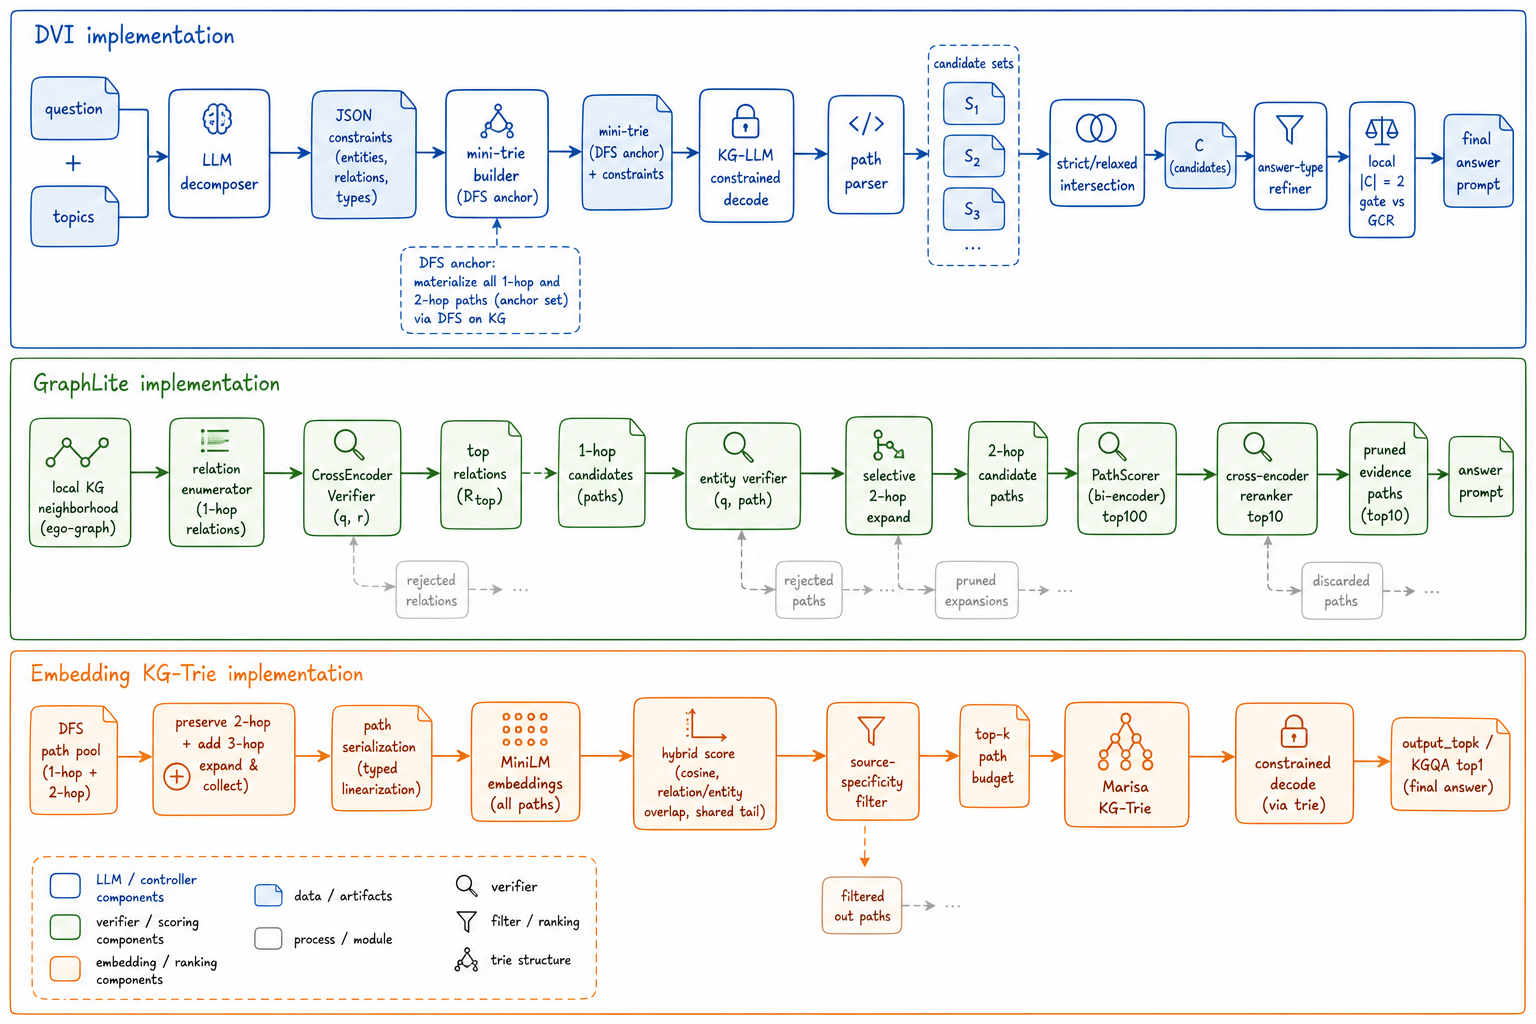
\includegraphics[width=\textwidth,height=0.48\textheight,keepaspectratio]{method_architecture_implementation_blueprint_gpt-image-2-v5.png}
\caption{Implementation-level method architecture. Unlike the project overview, this figure expands each method into internal modules, intermediate data structures, and control decisions: DVI tracks constraints and candidate sets, GraphLite replaces KG-LLM decoding with relation/entity/path verifiers, and embedding-guided KG-Trie ranks and budgets paths before trie construction.}
\label{fig:method-architectures}
\end{figure*}

\subsection{Worked Question-to-Answer Trace}
Figure~\ref{fig:q2a-trace} compares the three method-specific traces on one compositional question: ``The national anthem Afghan National Anthem is from the country which practices what religions?'' The correct trace is not a single topical path about the anthem. It must bind the anthem to its country, keep the target answer type as \emph{religion}, and then return the religions connected to that country: \emph{Sunni Islam} and \emph{Shia Islam}.

\begin{figure*}[t]
\centering
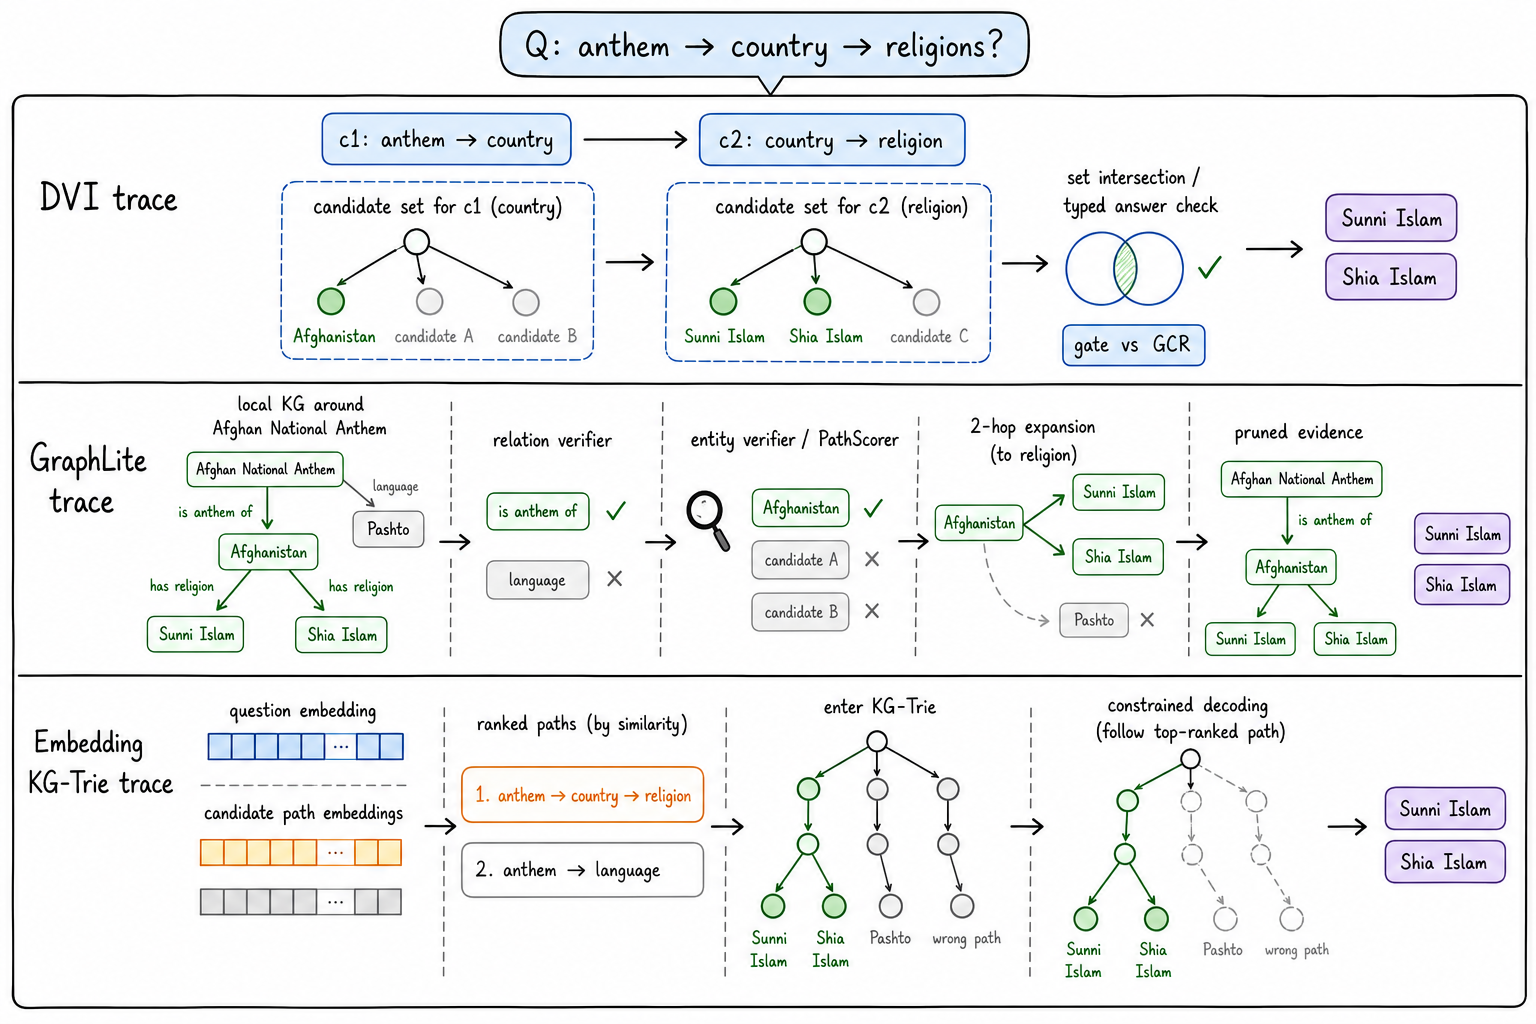
\includegraphics[width=\textwidth,height=0.38\textheight,keepaspectratio]{three_method_traces_gpt-image-2-v3.png}
\caption{Three separate question-to-answer traces for the same anthem-country-religion query. DVI traces decomposition and candidate intersection, GraphLite traces relation/entity verification and pruning, and embedding-guided KG-Trie traces semantic path ranking before constrained decoding.}
\label{fig:q2a-trace}
\end{figure*}

In DVI terms, the decomposer should produce two relation constraints, anthem $\rightarrow$ country and country $\rightarrow$ religion. Mini-tries verify each branch, the bridge country candidate is carried forward, and answer-aware refinement checks that final candidates are religions. In GraphLite terms, relation and entity verifiers should downweight the tempting but wrong language path and keep country/religion paths. In embedding-guided KG-Trie terms, semantic ranking should keep the country/religion evidence in the trie while preventing generic music-language paths from dominating the constrained decoder.

\section{Implementation Details}
The implementation keeps DVI, GraphLite, and embedding-guided KG-Trie as separate code paths so that failures can be attributed to the controller, verifier, or trie-construction stage. DVI prediction files store both answers and metadata: decomposition status, relation/filter constraints, per-constraint path counts, trie statistics, strict and relaxed intersection sizes, candidate sets, fallback mode, answer-type hints, and timing for decomposition, KG decoding, path scoring, intersection, and final answering. This metadata is what makes post-hoc routed DVI possible without rerunning the KG model.

Two engineering choices matter most. First, DVI uses selective fallback: if a question has only one relation constraint or decomposition fails on a single-topic example, the system keeps the original global GCR trie instead of forcing mini-tries that have no intersection advantage. Second, embedding-guided KG-Trie separates the number of DFS paths collected from the number admitted into the trie; on 3-hop CWQ probes, this budget is essential because raw candidate pools can exceed hundreds of thousands of paths. GraphLite changes the verifier side instead: it trades KG-LLM decoding for explicit graph enumeration plus relation/entity/path scoring, which explains the much lower runtime and the current quality drop.

\section{Experimental Setup}
We evaluate mainly on RoG-CWQ. The full test split contains 3531 examples. We also use RoG-WebQSP to test whether embedding-guided path selection transfers to a simpler KGQA benchmark. Metrics are Precision, Recall, F1, Hit@1, and Hit. The archived evaluation script also reports Accuracy, which aligns with answer-set recall in these outputs. Timing is mean wall-clock seconds per example when prediction files contain timing metadata.

The reproduced full CWQ baselines use hop length 2, zero-shot group beam search, $k=10$, and GPT-4o mini as the final answer LLM. We compare three KG-specialized LLM checkpoints: Llama-3.1-8B, Llama-2-7B, and Qwen2-0.5B~\cite{grattafiori2024llama3,touvron2023llama2,yang2024qwen2}. Embedding-guided GCR uses Qwen2-0.5B for method-only comparison and Meta-Llama-3.1-8B for base-model exploration. DVI uses both Llama-3.1 and Llama-2, plus a Qwen ablation. GraphLite uses the PathScorer verifier without a KG-specialized generation model.

\section{Main Results}
\begin{table*}[t]
\centering
\small
\resizebox{\textwidth}{!}{
\begin{tabular}{llrrrrrrrr}
\toprule
Method & KG/verifier & N & Acc./Rec. & Hit & Hit@1 & F1 & Prec. & Time(s) & Coverage \\
\midrule
GCR baseline & Llama-3.1-8B & 3531 & 59.01 & 64.34 & 55.88 & 54.55 & 54.87 & 2.06 & 882/3531 \\
GCR baseline & Llama-2-7B & 3531 & 60.51 & 66.07 & \textbf{57.12} & 54.50 & 54.29 & 6.27 & 3531/3531 \\
GCR baseline & Qwen2-0.5B & 3531 & 47.81 & 54.46 & 44.83 & 42.31 & 42.52 & 1.68 & 3531/3531 \\
\midrule
Raw DVI & Llama-3.1-8B & 3520 & 57.71 & 64.32 & 54.18 & 52.57 & 53.42 & 12.72 & 3520/3520 \\
Routed DVI, $|C|=2$ & Llama-3.1-8B & 3531 & 59.26 & 64.68 & 56.22 & \textbf{54.63} & \textbf{54.90} & 6.58 & 1307/3531 \\
Raw DVI & Llama-2-7B & 3520 & 57.76 & 64.35 & 53.86 & 52.31 & 53.02 & 7.92 & 3520/3520 \\
Routed DVI, $|C|=2$ & Llama-2-7B & 3531 & \textbf{60.56} & \textbf{66.27} & 56.92 & 54.51 & 54.42 & 6.53 & 3531/3531 \\
\midrule
GraphLite / PathScorer & Entity / path verifier & 3520 & 51.05 & 56.19 & 45.09 & 42.14 & 40.64 & \textbf{3.09} & 3520/3520 \\
\bottomrule
\end{tabular}}
\caption{Full-test RoG-CWQ results. Values are percentages except time. Routed DVI uses DVI only when the final candidate set has exactly two entities; otherwise it keeps the corresponding GCR prediction.}
\label{tab:main}
\end{table*}

Table~\ref{tab:main} gives the full-test results. The three reproduced GCR baselines satisfy the project requirement to explore more than two KG-specialized LLMs. Llama-2 has the strongest Accuracy/Recall, Hit, and Hit@1; Llama-3.1 has the strongest baseline F1 and Precision; Qwen2-0.5B is much faster and weaker.

Raw DVI does not beat the strongest GCR baselines. It has useful examples, but the full DVI pipeline is vulnerable to decomposition mistakes and answer-incomplete mediator endpoints. Exact-size routed DVI is more stable. For Llama-3.1, it improves Accuracy/Recall from 59.01 to 59.26, Hit from 64.34 to 64.68, Hit@1 from 55.88 to 56.22, F1 from 54.55 to 54.63, and Precision from 54.87 to 54.90. For Llama-2, it improves Accuracy/Recall from 60.51 to 60.56, Hit from 66.07 to 66.27, F1 from 54.50 to 54.51, and Precision from 54.29 to 54.42, while lowering Hit@1 from 57.12 to 56.92. These gains are small, so the result should be interpreted as evidence for a useful routing direction rather than a decisive leaderboard improvement.

GraphLite is the fastest full-test verifier among our modified methods. It reduces mean inference time from 12.72s for Llama-3.1 raw DVI to 3.09s, but F1 drops from 52.57 to 42.14. This makes GraphLite useful as an efficiency ablation and possible prefilter, but not yet a replacement for KG-LLM verification.

\subsection{Oracle Routing Headroom}
The strongest evidence for DVI is complementarity. On the 3520 examples shared by the Llama-3.1 baseline and raw DVI, a post-hoc oracle that chooses the prediction source with higher F1 reaches 61.51 F1, compared with 54.63 for the baseline on the same examples and 52.57 for raw DVI. DVI uniquely fixes 282 Hit@1 examples that GCR misses, while GCR uniquely fixes 348 that DVI misses. Llama-2 shows the same pattern: oracle F1 reaches 61.37, with 259 DVI-only Hit@1 fixes and 379 baseline-only fixes. This means DVI contains useful signal, but a better learned router is needed.

\begin{table}[H]
\centering
\small
\resizebox{\columnwidth}{!}{
\begin{tabular}{llrrrr}
\toprule
KG model & Source & N & Hit@1 & F1 & Hit \\
\midrule
Llama-3.1 & GCR & 3520 & 56.05 & 54.63 & 64.43 \\
Llama-3.1 & Raw DVI & 3520 & 54.18 & 52.57 & 64.32 \\
Llama-3.1 & Oracle & 3520 & \textbf{62.36} & \textbf{61.51} & \textbf{71.45} \\
\midrule
Llama-2 & GCR & 3520 & 57.27 & 54.57 & 66.16 \\
Llama-2 & Raw DVI & 3520 & 53.86 & 52.31 & 64.35 \\
Llama-2 & Oracle & 3520 & \textbf{63.35} & \textbf{61.37} & \textbf{72.39} \\
\bottomrule
\end{tabular}
}
\caption{Post-hoc oracle routing over shared GCR/DVI examples. This is an upper bound, not a deployable method.}
\label{tab:oracle}
\end{table}

\section{Embedding-Guided KG-Trie Results}
\begin{table*}[t]
\centering
\small
\resizebox{\textwidth}{!}{
\begin{tabular}{lllrrrr}
\toprule
Dataset & Method & Setting & Acc./Rec. & Hit & F1 & Precision \\
\midrule
CWQ full & Qwen GCR & 2-hop baseline & 55.60 & 62.50 & \textbf{23.86} & 17.73 \\
CWQ full & Qwen embedding & 2-hop baseline-aligned & 55.48 & 62.39 & 23.76 & 17.66 \\
WebQSP full & Qwen GCR & 2-hop baseline & 68.39 & 87.71 & \textbf{37.17} & 33.58 \\
WebQSP full & Qwen embedding & 2-hop baseline-aligned & 67.75 & 87.77 & 36.87 & 33.44 \\
\midrule
CWQ100 & preserve-2 + emb-3 & all candidates & 63.42 & 70.00 & 27.48 & 20.27 \\
CWQ100 & baseline + emb-3 fusion & KGQA top-1 & 39.13 & 47.00 & \textbf{39.68} & \textbf{45.00} \\
WebQSP100 & preserve-2 + emb-3 & all candidates & 70.89 & 90.00 & 34.18 & 31.02 \\
WebQSP100 & preserve-2 + emb-3 & no-topic top-1 & 42.76 & 66.00 & \textbf{44.70} & \textbf{64.00} \\
CWQ20 & 3-hop embedding & output top-1 & 43.79 & 55.00 & \textbf{45.56} & \textbf{55.00} \\
\bottomrule
\end{tabular}}
\caption{Embedding-guided KG-Trie results. Pure 2-hop embedding selection is close to, but does not beat, the full Qwen baseline. It becomes useful when 2-hop coverage is preserved and 3-hop evidence is added with candidate reranking.}
\label{tab:embedding}
\end{table*}

Table~\ref{tab:embedding} summarizes the embedding line. The first full-test attempt simply inserted semantic ranking into 2-hop KG-Trie construction. This nearly ties the Qwen baseline but does not improve it: CWQ F1 is 23.76 vs. 23.86, and WebQSP F1 is 36.87 vs. 37.17. This negative result is informative: semantic similarity should not replace strong short-hop graph coverage.

The improved setting keeps 2-hop coverage and uses embedding ranking to add 3-hop evidence. On CWQ100, full candidates improve slightly in recall-style metrics, but the real gain appears after candidate fusion and KGQA-aware top-1 selection, reaching 39.68 F1. On WebQSP100, preserve-2 plus 3-hop embedding improves no-topic top-1 selection from 41.60 F1 for the baseline probe to 44.70 F1. On the controlled CWQ20 experiment, 3-hop embedding-guided top-1 reaches 45.56 F1, compared with 30.50 F1 for the strongest 2-hop beam baseline and 22.37 F1 for naive 3-hop without embedding. The pattern is consistent: extra hops help only when path explosion is controlled.

\section{Failure Analysis}
\subsection{By Compositionality Type}
Table~\ref{tab:type} reports changes in percentage points for exact-size routed DVI against its own GCR baseline. Routed DVI helps Llama-3.1 on composition and comparative Hit@1, while superlative questions remain difficult. Llama-2 shows small gains on composition, comparative F1, and superlative F1, but loses on conjunction. This mixed picture explains why the aggregate gain is small: decomposition and intersection help some complex patterns but can also drop correct evidence when the constraint representation is incomplete.

\begin{table}[H]
\centering
\small
\begin{tabular}{lrrrrr}
\toprule
Type & N & \multicolumn{2}{c}{Llama-3.1 $\Delta$} & \multicolumn{2}{c}{Llama-2 $\Delta$} \\
\cmidrule(lr){3-4}\cmidrule(lr){5-6}
 & & Hit@1 & F1 & Hit@1 & F1 \\
\midrule
composition & 1546 & +0.84 & +0.55 & +0.19 & +0.26 \\
conjunction & 1575 & -0.19 & -0.12 & -0.76 & -0.38 \\
comparative & 213 & +1.88 & -0.01 & +0.94 & +0.70 \\
superlative & 197 & -1.02 & -1.92 & +0.00 & +0.54 \\
\bottomrule
\end{tabular}
\caption{Compositionality-type change for exact-size routed DVI versus the corresponding GCR baseline.}
\label{tab:type}
\end{table}

\subsection{Detailed Failure Inference Steps}
The rubric asks for detailed inference steps on multi-constraint failures. Table~\ref{tab:failure-steps} gives representative examples from the archived predictions and shows exactly which step breaks. The common pattern is that the generated paths are KG-valid, but the system either starts from a generic topic entity, follows the wrong relation, or fails to execute an intersection or filter.

\begin{table*}[t]
\centering
\small
\begin{tabular}{p{0.18\textwidth}p{0.27\textwidth}p{0.30\textwidth}p{0.18\textwidth}}
\toprule
Case & Required inference steps & Observed KG-valid path / output & Failure point \\
\midrule
Country Nation World Tour college &
1. Find the artist of \emph{Country Nation World Tour}. 2. Follow the artist's education relation. 3. Return the institution, gold \emph{Belmont University}. &
The model follows a generic type source: \emph{College/University $\rightarrow$ College $\rightarrow$ films $\rightarrow$ Johnny Be Good $\rightarrow$ country $\rightarrow$ United States}. &
Generic-entity retrieval and answer-type failure. The path is valid but never identifies the tour artist. \\
\midrule
Afghan National Anthem religions &
1. Map the anthem to its country. 2. From that country, retrieve practiced religions. 3. Return \emph{Sunni Islam} and \emph{Shia Islam}. &
The model follows a topical but wrong relation: \emph{Afghan National Anthem $\rightarrow$ language $\rightarrow$ Pashto language}. Some paths continue to Afghanistan but return official language. &
Relation-selection failure. The path is about language rather than religion. \\
\midrule
Libya anthem leader &
1. Identify the country whose anthem is \emph{Libya, Libya, Libya}. 2. Intersect with the office/person constraint from \emph{Prime Minister of Libya}. 3. Return the leader, gold \emph{Abdullah al-Thani}. &
Predicted paths include \emph{Prime Minister of Libya $\rightarrow$ office holders $\rightarrow$ position record $\rightarrow$ jurisdiction $\rightarrow$ Libya $\rightarrow$ languages spoken $\rightarrow$ Arabic}. &
Aggregation and typing failure. The system reaches Libya but drifts to language, not the office holder. \\
\midrule
Alta Verapaz and Central America &
1. Candidate country must contain \emph{Alta Verapaz Department}. 2. Candidate must also be in \emph{Central America}. 3. Return the intersection, gold \emph{Guatemala}. &
Baseline follows paths from generic \emph{Country}, e.g., fictional country settings ending in \emph{Europe}. &
Multi-entity intersection failure. Generic paths overwhelm the specific department/region evidence. \\
\midrule
Temporal governor filter &
1. Retrieve governors of Arizona. 2. Check who held office in 2009. 3. Apply the predicate ``held governmental position before 1998''. &
Graph paths can retrieve governor/office-holder candidates, but the date predicates are not executed by the trie. &
Operator failure. Prefix validity does not evaluate temporal constraints. \\
\bottomrule
\end{tabular}
\caption{Detailed inference-step failures. Each error is KG-valid at the path level but invalid at the full-question constraint level.}
\label{tab:failure-steps}
\end{table*}

The first and fourth rows motivate embedding-guided path selection: generic sources such as \emph{Country} or \emph{College/University} create many valid distractors, so semantic ranking and generic-source filtering are useful. The second row motivates relation-aware scoring: topic similarity alone is insufficient because the anthem-language path is semantically close but predicate-wrong. The third row motivates DVI: multiple topic entities must be combined through answer-level intersection rather than left to the final LLM. The fifth row is the main remaining gap: neither DVI nor GraphLite fully executes temporal and numeric filters yet.

\subsection{Error Taxonomy Across Methods}
The failure cases can be organized by which part of the pipeline failed.

\paragraph{Retrieval failure.}
The needed entity or relation path is absent from the local path pool. This happens when the hop limit is too small, when the relevant bridge is beyond the DFS budget, or when topic entity linking gives a generic type node. Embedding-guided 3-hop expansion primarily targets this failure mode.

\paragraph{Selection failure.}
The correct path exists in the pool but is ranked below distractors. GraphLite and embedding-guided ranking both target this failure mode. The path-reranker training results show that supervised scoring can substantially improve path-level Hit@1, but QA still requires downstream aggregation.

\paragraph{Aggregation failure.}
The evidence contains paths for several constraints, but the system fails to combine them into a single answer. This is the main motivation for DVI. GCR leaves most aggregation to the final LLM; DVI turns at least the entity-intersection part into deterministic Python set operations.

\paragraph{Typing failure.}
The system finds a related entity but not an entity of the requested answer type. Examples include returning a language when the question asks for a religion, a country when it asks for a currency, or a mediator record when it asks for a person. Answer-aware refinement targets this failure mode, but the current rules are incomplete.

\paragraph{Operator failure.}
The system retrieves candidates that satisfy relation constraints but does not execute date, numeric, comparative, or superlative operators. This failure mode remains mostly unsolved in the current implementation. It requires compiling filters into executable comparisons over KG attributes.

This taxonomy explains why the methods are complementary. Embedding-guided KG-Trie helps retrieval and selection, GraphLite helps selection and speed, and DVI helps aggregation. None of them fully solves typing and operator execution yet.

\section{Ablation and Hyperparameter Analysis}
The project rubric requires ablations beyond the main-result table. We therefore keep the main ablation tables in the body and use them to diagnose calibration, verifier quality, and path-budget sensitivity.

\subsection{DVI Gate Thresholds}
Table~\ref{tab:gate} compares hand-written DVI confidence gates. Singleton DVI outputs often look precise but can be mediator endpoints, while broad gates reintroduce noisy alternatives. Exact-size routing, $|C|=2$, is the most stable deployed rule across the two stronger KG-specialized LLMs.

\begin{table}[H]
\centering
\scriptsize
\resizebox{\columnwidth}{!}{
\begin{tabular}{llrrrr}
\toprule
Model & Gate & Acc./Rec. & Hit@1 & F1 & Time(s) \\
\midrule
Llama-3.1 & $|C|\le1$ & 59.03 & 54.80 & 54.33 & 8.54 \\
Llama-3.1 & $|C|=2$ & 59.26 & 56.22 & \textbf{54.63} & 6.58 \\
Llama-3.1 & $|C|\le2$ & \textbf{59.28} & 55.14 & 54.41 & 10.29 \\
Llama-3.1 & $|C|\le3$ & 58.92 & 54.63 & 53.87 & 11.27 \\
\midrule
Llama-2 & $|C|\le1$ & 60.40 & 55.88 & 54.38 & 6.89 \\
Llama-2 & $|C|=2$ & \textbf{60.56} & \textbf{56.92} & \textbf{54.51} & 6.53 \\
Llama-2 & $|C|\le2$ & 60.45 & 55.68 & 54.40 & 7.16 \\
Llama-2 & $|C|\le3$ & 59.71 & 54.91 & 53.84 & 7.34 \\
\bottomrule
\end{tabular}}
\caption{DVI confidence-gate ablation. Exact-size routing is the most stable threshold across the two stronger KG-specialized LLMs.}
\label{tab:gate}
\end{table}

\subsection{GraphLite Verifier Training}
GraphLite tests whether expensive KG-LLM verification can be replaced by explicit path enumeration and neural scoring. Fine-tuning the cross-encoder improves path-level ranking, but endpoint supervision still does not guarantee full answer satisfaction.

\begin{table}[H]
\centering
\scriptsize
\resizebox{\columnwidth}{!}{
\begin{tabular}{lrrrrr}
\toprule
Verifier & Groups & MRR & Hit@1 & Hit@5 & Hit@10 \\
\midrule
Pretrained cross-encoder & 158 & 68.04 & 56.33 & 85.44 & 88.61 \\
Fine-tuned cross-encoder & 158 & \textbf{77.13} & \textbf{69.62} & \textbf{87.97} & \textbf{91.77} \\
\bottomrule
\end{tabular}}
\caption{GraphLite path-reranker training metrics on held-out grouped path candidates. Values are percentages except group count.}
\label{tab:graphlite-training}
\end{table}

\subsection{Hop Length and Candidate Selection}
Embedding-guided KG-Trie has the opposite calibration problem: extra hops improve coverage but create many distractors. Table~\ref{tab:hop-ablation} shows that naive 3-hop expansion hurts, while embedding-guided selection makes 3-hop evidence useful.

\begin{table}[H]
\centering
\scriptsize
\resizebox{\columnwidth}{!}{
\begin{tabular}{lrrrr}
\toprule
CWQ20 setting & Hit & F1 & Prec. & Recall \\
\midrule
2-hop group-beam baseline & 45.00 & 27.83 & 30.00 & 36.88 \\
2-hop beam early stopping & 45.00 & 30.50 & 34.17 & 36.88 \\
3-hop budgeted, no embedding & 45.00 & 22.37 & 20.83 & 31.29 \\
3-hop embedding, all candidates & \textbf{60.00} & 37.00 & 37.50 & \textbf{51.88} \\
3-hop embedding, top-1 & 55.00 & \textbf{45.56} & \textbf{55.00} & 43.79 \\
\bottomrule
\end{tabular}}
\caption{Hop-length and output-selection ablation on CWQ20. Extra hops help only when semantic selection and candidate filtering control path explosion.}
\label{tab:hop-ablation}
\end{table}

Across the ablations, the recurring pattern is calibration: DVI needs calibrated routing, GraphLite needs calibrated verifier scores, and embedding-guided KG-Trie needs calibrated path budgets.

\section{Discussion}
The results support four conclusions.

First, GCR is a strong baseline and the KG-specialized model matters. Llama-2 and Llama-3.1 are far stronger than Qwen2-0.5B on final-answer CWQ metrics. This satisfies the base-LLM exploration requirement and also shows that method comparisons must control for model capacity.

Second, DVI should be selective. Raw DVI has useful answers but is not robust enough to replace GCR globally. Exact-size gating gives small full-test gains, while oracle routing shows large headroom. The next version should train a router from DVI metadata, question type, candidate count, strict-intersection size, relaxation status, answer type, and baseline confidence.

Third, GraphLite exposes the speed-quality frontier. Explicit relation/entity enumeration plus neural scoring is much faster than KG-LLM DVI, but loses quality. Fine-tuned path reranking improves grouped verifier Hit@1 from 56.33\% to 69.62\% on held-out path groups, yet QA performance remains below the strongest GCR/DVI methods. This suggests GraphLite is best used as a prefilter or auxiliary verifier, not a standalone answer system.

Fourth, embedding-guided KG-Trie is a useful path-construction module only when coverage is protected. Pure 2-hop semantic pruning is too aggressive; preserve-2 plus 3-hop embedding expansion is more promising. The method is complementary to DVI because it improves the evidence pool, while DVI improves constraint aggregation.

\section{Limitations and Future Work}
The current system is a working prototype rather than a finished KGQA solver. Its main limitations are answer typing, executable filters, and routing calibration. Answer-aware refinement uses lightweight type heuristics and local expansion, but a stronger system should learn answer types and mediator schemas. Temporal, numeric, comparative, and superlative questions require executable operators over KG attributes; the current DVI decomposer records these filters but mostly treats them as metadata. Routing is also still simple: exact-size gating gives a small full-test gain, while the oracle shows much larger headroom. A learned router should use decomposition status, strict-intersection size, relaxation status, fallback mode, answer-type confidence, path-score margins, and baseline confidence.

The three methods should eventually be merged into one configurable pipeline. Embedding-guided KG-Trie can expand evidence beyond 2 hops, GraphLite can cheaply score and prune paths, and DVI can perform deterministic intersection and answer-type validation. A stronger evaluation should report confidence intervals, evaluate CWQ and WebQSP under the same final-answer protocol, and isolate gains on examples requiring multi-entity intersection, date comparison, or superlative choice.


\paragraph{Integration plan.}
The next version should combine the three methods without adding a project-level router. A coverage-preserving evidence pool would keep the original 2-hop GCR neighborhood, add only embedding-ranked 3-hop paths, and store metadata such as source entity, hop length, relation overlap, embedding margin, and generic-source flags. GraphLite can then score this pool before KG-LLM decoding, producing compact accepted and rejected evidence paths. DVI can consume those paths as constraint-specific candidate sets, run strict or relaxed intersections, and expose routing features such as parse status, path counts, candidate-set size, relaxation depth, answer-type confidence, GraphLite score margin, and embedding-rank margin.

\paragraph{Remaining execution gap.}
The combined pipeline would still need a small executor for temporal, numeric, comparative, and superlative filters. The current trie/verifier stack checks graph validity and relation satisfaction, but it does not compute argmax, date overlap, or numeric comparison. DVI filter constraints should therefore compile into deterministic KG-attribute operations before the final answer prompt, so the final LLM receives both evidence paths and checked operator results.

\section{Conclusion}
We reproduced GCR and implemented three modifications for complex KGQA: DVI, GraphLite, and embedding-guided KG-Trie construction. DVI adds explicit constraint decomposition, per-constraint verification, deterministic candidate intersection, and confidence-gated routing. GraphLite studies a faster verifier based on entity-level graph enumeration and neural scoring. Embedding-guided KG-Trie changes trie construction so that semantically relevant 3-hop evidence can enter the decoder without uncontrolled path explosion.

The main empirical result is conservative but useful: exact-size routed DVI slightly improves the strongest reproduced GCR baselines, while oracle routing shows that DVI and GCR have substantial complementarity. GraphLite is faster but currently lower quality. Embedding-guided path selection improves controlled 3-hop probes but does not beat the full 2-hop Qwen baseline by itself. The main research lesson is that KG path validity is only the first layer of faithful reasoning. Complex KGQA needs explicit state for constraint coverage, answer type, entity intersection, and executable temporal, numeric, and superlative operators.

\section*{Individual Contributions}
\begin{itemize}
  \item \textbf{Member 1}: baseline reproduction, environment setup, model downloads, and full-test shard execution.
  \item \textbf{Member 2}: DVI controller, GraphLite/PathScorer verifier, routing experiments, and timing analysis.
  \item \textbf{Member 3}: embedding-guided KG-Trie implementation, failure analysis, report writing, and poster preparation.
\end{itemize}


\clearpage
\begin{thebibliography}{99}
\bibitem{berant2013semantic}
Jonathan Berant, Andrew Chou, Roy Frostig, and Percy Liang. 2013.
Semantic parsing on Freebase from question-answer pairs. EMNLP.

\bibitem{devlin2019bert}
Jacob Devlin, Ming-Wei Chang, Kenton Lee, and Kristina Toutanova. 2019.
BERT: Pre-training of deep bidirectional transformers for language understanding. NAACL.

\bibitem{grattafiori2024llama3}
Aaron Grattafiori et al. 2024.
The Llama 3 Herd of Models. arXiv.

\bibitem{he2021deberta}
Pengcheng He, Xiaodong Liu, Jianfeng Gao, and Weizhu Chen. 2021.
DeBERTa: Decoding-enhanced BERT with disentangled attention. ICLR.

\bibitem{jiang2023structgpt}
Jinhao Jiang, Kun Zhou, Zican Dong, Keming Ye, Xin Zhao, and Ji-Rong Wen. 2023.
StructGPT: A general framework for large language model to reason over structured data. arXiv.

\bibitem{lewis2020rag}
Patrick Lewis, Ethan Perez, Aleksandra Piktus, Fabio Petroni, Vladimir Karpukhin, Naman Goyal, Heinrich Kuettler, Mike Lewis, Wen-tau Yih, Tim Rocktaschel, Sebastian Riedel, and Douwe Kiela. 2020.
Retrieval-augmented generation for knowledge-intensive NLP tasks. NeurIPS.

\bibitem{luo2024rog}
Linhao Luo et al. 2024.
Reasoning on graphs: Faithful and interpretable large language model reasoning. ICLR.

\bibitem{luo2025gcr}
Linhao Luo, Zicheng Zhao, Gholamreza Haffari, Yuan-Fang Li, Chen Gong, and Shirui Pan. 2025.
Graph-constrained Reasoning: Faithful Reasoning on Knowledge Graphs with Large Language Models. ICML.

\bibitem{miller2016kvmem}
Alexander Miller et al. 2016.
Key-value memory networks for directly reading documents. EMNLP.

\bibitem{reimers2019sentencebert}
Nils Reimers and Iryna Gurevych. 2019.
Sentence-BERT: Sentence embeddings using Siamese BERT-networks. EMNLP-IJCNLP.

\bibitem{sun2018graftnet}
Haitian Sun, Bhuwan Dhingra, Manzil Zaheer, Kathryn Mazaitis, Ruslan Salakhutdinov, and William Cohen. 2018.
Open domain question answering using early fusion of knowledge bases and text. EMNLP.

\bibitem{sun2019pullnet}
Haitian Sun, Tania Bedrax-Weiss, and William Cohen. 2019.
PullNet: Open domain question answering with iterative retrieval on knowledge bases and text. EMNLP.

\bibitem{sun2023tog}
Jiashuo Sun et al. 2023.
Think-on-Graph: Deep and responsible reasoning of large language model on knowledge graph. arXiv.

\bibitem{talmor2018cwq}
Alon Talmor and Jonathan Berant. 2018.
The Web as a Knowledge-base for Answering Complex Questions. NAACL.

\bibitem{touvron2023llama2}
Hugo Touvron et al. 2023.
Llama 2: Open foundation and fine-tuned chat models. arXiv.

\bibitem{wang2020minilm}
Wenhui Wang, Furu Wei, Li Dong, Hangbo Bao, Nan Yang, and Ming Zhou. 2020.
MiniLM: Deep self-attention distillation for task-agnostic compression of pre-trained transformers. NeurIPS.

\bibitem{wang2023selfconsistency}
Xuezhi Wang et al. 2023.
Self-consistency improves chain of thought reasoning in language models. ICLR.

\bibitem{wei2022cot}
Jason Wei et al. 2022.
Chain-of-thought prompting elicits reasoning in language models. NeurIPS.

\bibitem{yang2024qwen2}
An Yang et al. 2024.
Qwen2 Technical Report. arXiv.

\bibitem{yao2023react}
Shunyu Yao et al. 2023.
ReAct: Synergizing reasoning and acting in language models. ICLR.

\bibitem{yih2016webqsp}
Wen-tau Yih, Matthew Richardson, Christopher Meek, Ming-Wei Chang, and Jina Suh. 2016.
The value of semantic parse labeling for knowledge base question answering. ACL.
\end{thebibliography}

\clearpage
\appendix

\section{Appendix: Reproducibility and Extra Details}
\small
This appendix contains material that supports the main ten-page report but is not required for the core narrative.

\subsection{Code Locations}
\begin{itemize}
  \item DVI implementation: \path{gcr-dvi/workflow/predict_dvi.py}, \path{gcr-dvi/src/dvi/decomposer.py}, \path{gcr-dvi/src/dvi/intersector.py}, \path{gcr-dvi/src/dvi/answer_aware.py}, and \path{gcr-dvi/src/qa_prompt_builder.py}.
  \item GraphLite entity-level prototype: \path{lite_framework.rar}, containing \path{entity_level_decoder.py}, \path{cross_encoder_verifier.py}, \path{graph_walker.py}, \path{graph_encoder.py}, \path{train_cross_encoder.py}, and \path{train_entity_verifier.py}.
  \item Integrated GraphLite / PathScorer implementation: \path{gcr-dvi/src/dvi/path_scorer.py}, \path{gcr-dvi/workflow/build_path_verifier_data.py}, and \path{gcr-dvi/workflow/train_path_reranker.py}.
  \item Embedding-guided KG-Trie implementation: \path{archive/20260509_keep_graph_code/custom_code/kgtrie_enhanced_mods/overlay/src/qa_prompt_builder.py} and \path{archive/20260509_keep_graph_code/custom_code/kgtrie_enhanced_mods/overlay/workflow/predict_paths_and_answers.py}.
  \item Main DVI results: \path{submission_20260510/results/DVI_v2_merged/}, \path{submission_20260510/results/DVI_v2_hybrid/}, and \path{submission_20260510/results/DVI_scorer_baseline_aligned/}.
  \item Main embedding results: \path{archive/20260509_keep_graph_code/experiment_results/enhanced_baseline_aligned_*}, \path{kgtrie_v2_cwq100_*}, and \path{kgtrie_v2_webqsp100_*}.
\end{itemize}

\subsection{DVI Gate Ablation}
\begin{table}[H]
\centering
\small
\begin{tabular}{llrrrr}
\toprule
Model & Gate & Acc./Rec. & Hit@1 & F1 & Time(s) \\
\midrule
Llama-3.1 & $|C|\le1$ & 59.03 & 54.80 & 54.33 & 8.54 \\
Llama-3.1 & $|C|=2$ & 59.26 & 56.22 & 54.63 & 6.58 \\
Llama-3.1 & $|C|\le2$ & 59.28 & 55.14 & 54.41 & 10.29 \\
Llama-3.1 & $|C|\le3$ & 58.92 & 54.63 & 53.87 & 11.27 \\
\midrule
Llama-2 & $|C|\le1$ & 60.40 & 55.88 & 54.38 & 6.89 \\
Llama-2 & $|C|=2$ & 60.56 & 56.92 & 54.51 & 6.53 \\
Llama-2 & $|C|\le2$ & 60.45 & 55.68 & 54.40 & 7.16 \\
Llama-2 & $|C|\le3$ & 59.71 & 54.91 & 53.84 & 7.34 \\
\bottomrule
\end{tabular}
\caption{DVI confidence-gate ablation. Exact-size routing is the most stable setting in this archive.}
\end{table}

\subsection{GraphLite Training Signal}
The trained cross-encoder path reranker improves held-out grouped path retrieval before QA: Hit@1 rises from 56.33\% to 69.62\%, MRR from 0.680 to 0.771, and Hit@10 from 88.61\% to 91.77\%. A 100-example QA probe with the trained scorer reaches 50.55 F1, and a post-hoc evidence setting reaches 53.52 F1. This improves over random or untrained path selection but remains below full KG-LLM DVI and strong GCR baselines.

\subsection{Additional Embedding Ablations}
On CWQ20, the 2-hop group-beam baseline has 27.83 F1, 2-hop beam early stopping has 30.50 F1, naive 3-hop with a path budget has 22.37 F1, and 3-hop embedding-guided top-1 reaches 45.56 F1. Hybrid lexical and structural scoring matches pure embedding in the best small setting but does not clearly exceed it. The main practical lesson is to protect short-hop coverage and use semantic ranking only to add evidence, not to prune the entire graph neighborhood aggressively.

\subsection{Failure Case Details}
\paragraph{College question.} Question: ``Where did the Country Nation World Tour concert artist go to college?'' Gold: Belmont University. The baseline often follows generic paths from \emph{College/University}; embedding sometimes retrieves more related paths but still predicts broad entities such as United States of America. A correct system must identify the concert artist and then follow the education relation to the institution.

\paragraph{Afghan National Anthem question.} Question: ``The national anthem Afghan National Anthem is from the country which practices what religions?'' Gold: Sunni Islam and Shia Islam. Generated paths often follow music-language relations and return Pashto language. This is a relation-mismatch failure: the path is related to the anthem but not to the asked religion predicate.

\paragraph{Libya anthem question.} Question: ``Which man is the leader of the country that uses Libya, Libya, Libya as its national anthem?'' Gold: Abdullah al-Thani. The system retrieves paths to Libya and prime-minister entities but returns generic roles or languages. This is a multi-entity intersection plus answer-type failure.

\subsection{Main Result Files}
\begin{itemize}
  \item GCR baselines: \path{submission_20260510/results/combined_baselines/RoG-cwq/}.
  \item Raw DVI full-test outputs: \path{submission_20260510/results/DVI_v2_merged/RoG-cwq/}.
  \item Routed DVI full-test outputs: \path{submission_20260510/results/DVI_v2_hybrid/RoG-cwq/}.
  \item GraphLite / PathScorer outputs: \path{submission_20260510/results/DVI_scorer_baseline_aligned/RoG-cwq/}.
\end{itemize}

\end{document}
